\documentclass[orivec]{llncs}
\usepackage{amsmath}
\usepackage{listings}
\usepackage{amsfonts}
\usepackage{graphicx}
\usepackage{courier}
\usepackage{algorithmic}
\usepackage[table,xcdraw]{xcolor}
\usepackage{float}
\usepackage{hyperref}
\usepackage{mathtools}
\usepackage[framemethod=TikZ]{mdframed}
\usepackage[]{inputenc}
\usepackage[T1]{fontenc}
\usepackage{placeins}
\usepackage{amsmath,amssymb}
\usepackage{xspace}

%to solve the hyperref problem of jumping to wrong places
\usepackage[all]{hypcap}
\usepackage[framemethod=TikZ]{mdframed}
\usepackage{fancyvrb}
\usepackage{relsize}
\graphicspath{{images/}}
\usepackage[boxruled,shortend,linesnumbered,algo2e]{algorithm2e}  % algo2e = use \begin{algorithm2e}
\usepackage{float}

\newcommand{\aeval}{\textsc{AE-VAL}\xspace}

\renewcommand{\labelitemi}{\tiny$\blacksquare$}

\newcommand{\andreas}[1]{\textcolor{blue}{Andreas: #1}}
\newcommand{\mike}[1]{\textcolor{red}{Mike: #1}}
\newcommand{\andrew}[1]{\textcolor{green}{Andrew: #1}}
\newcommand{\grigory}[1]{\textcolor{brown}{Grigory: #1}}

\newenvironment{requirement}
{\vspace{0.05in}
 \begin{mdframed}[roundcorner=10pt,backgroundcolor=gray!20]}
{\end{mdframed}}

\begin{document}

\title{Synthesis from Assume-Guarantee Contracts using Skolemized Proofs of
Realizability}
\author{Andreas Katis\inst{1}, Grigory Fedyukovich\inst{2}, Andrew
Gacek\inst{3}, John Backes\inst{3}, Michael W. Whalen\inst{1}}%
\institute{
Department of Computer Science and Engineering,\\
 University of Minnesota, 200 Union Street, Minneapolis, MN 55455,USA\\
\email{katis001@umn.edu, whalen@cs.umn.edu}
\and
Computer Science and Engineering, University of Washington, Seattle, Washington,
USA\\
\email{grigory@cs.washington.edu}
\and 
Rockwell Collins Advanced Technology Center\\
400 Collins Rd. NE, Cedar Rapids, IA, 52498, USA\\
\email{\{andrew.gacek,john.backes\}@rockwellcollins.com}
}
\maketitle

\begin{abstract}
In recent work, we proposed an extension of our realizability checking algorithm
for assume-guarantee contracts using theories. Given the k-inductive proof of a
contract's realizability, we use the power of a sophisticated skolemizer for
$\forall\exists$ formulas to construct an implementation composed of \textit{k}
skolem functions, guaranteed to comply to the user-defined requirements.
The algorithm is similar to k-induction model checking, but involves the use of 
quantifiers to determine realizability.

For the purposes of this paper we developed the proposed synthesis algorithm,
and successfully applied it to synthesize implementations for simple case
studies. We informally prove the algorithm's correctness and report our results
as well as the lessons that we learned during this experiment. Finally, we
discuss possible future directions that need to be explored to further improve the algorithm's application domain, optimality and efficiency.
\end{abstract}

\newcommand{\toolname}{RealSynth}

\mike{What should tool name be?  KindSyn, RealSyn, jsyn ``jason''.  I have defined it by command to make it easy to replace.}

\section{Introduction}
Automated synthesis research is concerned with discovering efficient algorithms to construct candidate programs that are guaranteed to comply with predefined temporal specifications.  This problem has been well studied for propositional specifications, especially for (subsets of) LTL~\cite{gulwani2010dimensions}.  More recently, the problem of synthesizing programs for richer theories has been examined, including work in {\em template synthesis}~\cite{srivastava2013template}, which attempts to find programs that match a certain shape (the template), and {\em inductive synthesis}, which attempts to use counterexample-based refinement to solve synthesis problems~\cite{flener2001inductive}.  Such techniques have been widely used for stateless formulas over arithmetic domains~\cite{reynoldscounterexample}.  
\textit{Functional synthesis} has also been effectively used to synthesize
subcomponents of already existing partial
implementations~\cite{kuncak2010complete,kuncak2013functional}. In this paper,
we propose a new approach that can synthesize programs for arbitrary {\em
assume/guarantee contracts} that do not have to conform to specific template
shapes or temporal restrictions. The contracts are described using
safety properties involving real arithmetic.  Although the
technique is not guaranteed to succeed or terminate, we have used it to successfully synthesize a range of programs over non-trivial contracts.
The power of expressiveness that is provided by the Assume-Guarantee framework
acts as the main catalyst behind the vast variety of applications that can be
supported by our synthesis procedure, involving instances from all of the
different research areas that were mentioned in the beginning of this Section.
As such, it can be used both with template-based specifications, support
temporal safety properties, potentially support counterexample refinement as an
intermediate optimization, as well as construct program fragments that
correspond to specification for leaf-level system components.

Our approach is built on previous work determining the {\em realizability} of contracts involving infinite theories such as linear integer/real arithmetic and/or uninterpreted functions~\cite{Katis15:Realizability,katis2015machine}.  The algorithm, explained in Section~\ref{sec:synthesis}, uses a quantified variant of k-induction that can be checked by any SMT solver that supports quantification.  Notionally, it checks whether a sequence of states satisfy the contract of depth $k$ is sufficient to guarantee the existence of a successor state that satisfies the contract for an arbitrary input.  An outer loop of the algorithm increases $k$ until either a solution or counterexample is found.  

The step from realizability to synthesis involves moving from the existence of a witness (as can be provided by an SMT solver such as z3 or cvc4) to the witness itself.  For this, the most important obstacle is the (in)ability of the SMT solver to handle higher-order quantification. Fortunately, interesting directions to solving this problem have already surfaced, either by extending an SMT solver with native synthesis capabilities\cite{reynoldscounterexample}, or by providing external algorithms that reduce the problem by efficient quantifier elimination methods~\cite{fedyukovichae}.  Our synthesis relies on our previous implementation for realizability checking and the skolemization procedure implemented in the AE-VAL tool~\cite{fedyukovichae}.


We combined the above ideas to create a reasonable sequential synthesis
approach, which we call \toolname.  It applies the realizability checker from~\cite{Katis15:Realizability} and then extracts a Skolem witness formula from the AE-VAL tool that can immediately be turned into a C program.  In order to support synthesis, several changes were required to the quantifier-elimination approach to produce Skolem {\em functions} rather than {\em relations}.  The main contributions of the work are therefore:
\begin{itemize}
	\item To the best of our knowledge, the first synthesis procedure from
	Assume-Guarantee contracts, modulo infinite theories, usable in a broader
	list of applications when compared to already existing approaches.
	\item \mike{GRIGORY: Something about improvements to AEVal to support synthesis}
	\item A prototype tool implementing the algorithm
	\item An experiment demonstrating the application of the tool on various benchmark examples
\end{itemize}

\noindent This paper presents the first full exposition of the idea, which was originally proposed in a workshop paper without an implementation or experiment~\cite{katis2016towards}.

In Section~\ref{sec:synthesis} we provide the necessary background
definitions that are used in our synthesis algorithm, as well as an informal
proof of the algorithm's correctness. Section~\ref{sec:aeval} contains the
core formal notions behind on which the AE-VAL Skolemizer is based, as well
as the adjustments that were done for it to better support the needs of this
work. Section~\ref{sec:impl} provides detailed
source information for each one of the important
components of this work. Section~\ref{sec:experiment} presents our results on
using the algorithm to automatically generate leaf-level component implementations for different case studies.
Finally, in Section~\ref{sec:related} we give a brief historical background on the related research work on synthesis, and we conclude with a discussion on potential future work in Section~\ref{sec:futurework}.

\iffalse



\grigory{The intro needs work. What's the main challenge? Why do we start with formal verification, and with synthesis or realizability checking?}
Formal verification is a well-established area of research, with ever increasing
popularity, in an attempt to provide better tools to software engineers during
the design and testing phases of a project and effectively reduce its overall
development cost. A particularly interesting problem in formal verification \grigory{this is not 100\% right, since program synthesis spreads far beyond program verification. There are many applications of synthesis that are not based on verification.} is
that of program synthesis aiming to construct efficient algorithms that can
automatically generate code which is guaranteed to behave correctly based on the
information provided by the user through formal or informal requirements.
\grigory{informal requirements? how come?}

Program synthesis has been applied in a significant amount of
diverse contexts, \grigory{citations?}, but to the best of our knowledge there is no application yet that ....%
 \grigory{what's the best novelty in our synthesis application?}
In this paper, we focus on the automated
generation of implementations for the leaf-level components of embedded
systems, using safety properties that are expressed in the form of an
Assume-Guarantee contract.
In recent work~\cite{katis2016towards}, we presented an idea for the Skolem-guided synthesis algorithm
that given a contract written in AADL would check realizability and derive an implementation,
but we did not implement it due to significant limitations in our Skolemizer~\cite{fedyukovich2015automated}.
\grigory{need to show other weaknesses of the previous work. Otherwise the reviewers may say ``not enough contributions''.}
%, can provide an implementation
%that is able to react to uncontrolled inputs provided by the system's
%environment, while satisfying the restrictions specified in the contract
%assumptions and guarantees.

The synthesis algorithm is an extension of our previous work on solving the problem of
realizability modulo infinite theories~\cite{Katis15:Realizability}, using a
model checking algorithm that has been formally verified in terms of its soundness for realizable
results~\cite{katis2015machine}.
\grigory{as we agreed earlier, there could be more description on k-induction}
 Given the inductive proof of realizability, we generate Skolem functions which are the
witnesses of strategies that a synthesized implementation can follow at each
step of execution.

\grigory{Let us invent a name for ``of our extension to \jkind's
realizability checking algorithm to support synthesis'' and use it everywhere.
The working name is \jkindsynt.}

We have implemented the synthesis
algorithm and exercised it in terms of its performance on several models. We
provide an informal proof of the algorithm's correctness regarding the
implementations that it produces, and discuss our experimental results.
\grigory{need more info here. some executive summary of the evaluation section.}

\fi
\newcommand{\realizable}{\textsc{realizable}}
\newcommand{\unrealizable}{\textsc{unrealizable}}
\newcommand{\skolems}{\textit{Skolems}}
\newcommand{\isValid}{\textsc{isValid}\xspace}
\newcommand{\isInvalid}{\textsc{isInvalid}\xspace}


% \newcommand{\synthesisalgorithm}{
% \begin{algorithm2e}[H]
% \SetAlFnt{\tiny}
% \SetAlCapFnt{\small}
% \SetAlCapNameFnt{\small}
% \SetAlgoSkip{}
% \SetKwFor{While}{forever}{do}{}
% \SetKw{KwContinue}{continue}
% \KwIn{Assume-Guarantee Contract in Lustre, $(A,G)$}
% \KwOut{Skolem collection \skolems, \\ \hspace{+1.3cm} Return value $\in
% \{\realizable, \unrealizable\}$ of ${(A,G)}$.
% }
% \BlankLine
% $i \gets 0$;\\
% $BaseResult \gets \textsc{BaseCheckEngine.\aeval}(BaseCheck(i))$\;
% $ExtendResult \gets \textsc{ExtendCheckEngine.\aeval}(ExtendCheck(i))$;
% \\
% \While{}{	
% 	\uIf(\label{alg:returnUnsat}){(\textsc{BaseCheckEngine}.\isValid($BaseResult$))}
% 	{
% 		\Return
% 		\unrealizable
% 	}
% 	$Skolems.Add(BaseResult.Skolem)$;\\
% 	\uIf(\label{alg:returnSat}){$(\textsc{ExtendCheckEngine}.\isInvalid($ExtendResult$))$}
% 	{
% 		$Skolems.Add((ExtendResult.Skolem))$;\\
% 		\Return \skolems, \realizable
% 	}
% 	$i$++;
% }
% \caption{Synthesis from Assume-Guarantee Contracts}
% \label{alg:synthesis}
% \end{algorithm2e}
% }


\section{Synthesis from Assume-Guarantee Contracts}
\label{sec:synthesis}

%GRIGORY: no need to repeat the things since they all are mentioned in the intro (a couple of paragraphs above)
%
In this section we provide %a summary of the formal background
%that has already been established in previous work, regarding an algorithm that
%is able to generate leaf-level component implementations using only the
%information provided by the user through requirements expressed in the form of an
%Assume-Guarantee contract. Our approach supports the Linear Real
%Arithmetic (LRA) theory.
%mainly due to the limitations imposed by the underlying machinery.
% We begin with
a brief background on Assume-Guarantee contracts,
proceed with summarizing our earlier results on realizability
checking of contracts, and finally
present our program synthesis procedure.
%Finally, we enrich our formal definitions with an informal proof of the
%algorithm's correctness in terms of the successfully synthesized
%implementations.

\subsection{Assume-Guarantee Contracts}

One popular way to describe software requirements is through Assume-Guarantee contracts, where requirements are expressed using safety properties that are split into two categories. The \emph{assumptions} of the contract correspond to properties that restrict the set of valid inputs a system can process, while the \emph{guarantees} dictate how the system should behave through constraints on the outputs that are produced by the system.

For example, consider the contract with the assumption $A = \{x\neq
y\}$ and the guarantee $G = \{x \leq y \Longrightarrow z =
\textit{true}, x \geq y \Longrightarrow z = \textit{false}\}$, for a component with two inputs $x$ and $y$ and one output $z$.  By assumption, $x \neq y$, so the implemented system should set $z$ to true if $x < y$ and false otherwise.  %Although this contract is trivial to implement, the contract does not provide an implementation, only a specification.
%
Determining whether an implementation can be constructed to satisfy the contract for all possible input sequences is the \emph{realizability} problem, while automatically constructing a witness of the proof of
realizability of the contract is the \emph{program synthesis} problem.  The contract $(A,G)$ above is obviously \emph{realizable}, and therefore an implementation can be constructed.
However, if the assumption is omitted then the contract is \emph{unrealizable}, since there is no correct value for $z$ when $x=y$.

\subsection{Formal Preliminaries}
\label{sec:pre}

We describe a system using the disjoint sets $state$ and $inputs$.
Formally, an \emph{implementation} is a \emph{transition system}
described by an initial state predicate $I(s)$ of type $state \to
bool$ and by a transition relation $T(s,i,s')$ of type $state \to
inputs \to state \to bool$.

An Assume-Guarantee (AG) contract can be formally defined by a set of
\emph{assumptions} and a set of \emph{guarantees}. The
\emph{assumptions}, $A: state \rightarrow inputs \rightarrow bool$,
impose constraints over the inputs which may be modal in terms of the
previous state. The \emph{guarantees} $G$ consist of two separate
subsets $G_I: state \rightarrow bool$ and $G_T: state \rightarrow
inputs \rightarrow state \rightarrow bool$, where $G_I$ defines the
set of valid initial states, and $G_T$ specifies the properties that
need to be met during each new transition between two states. Note
that we do not necessarily expect that a contract would be defined
over all variables in the transition system, but we do not make any
distinction between internal state variables and outputs in the
formalism. This way, we can use state variables to (in some cases)
simplify specification of guarantees.

\subsection{Realizability of Contracts}
The synthesis algorithm proposed in this paper is built on top of our realizability algorithm
originally presented in~\cite{Katis15:Realizability}. Using the formal foundations described in Sect.~\ref{sec:pre},
the problem of realizability is expressed using the notion of a state being \emph{extendable}:

\begin{definition}[One-step extension]
\label{def:extend}
A state $s$ is extendable after $n$ steps, denoted $\mathit{Extend}_{n}(s)$, if
any valid path of length $n-1$ starting from $s$ can be extended in response to
any valid input.%
%
\begin{multline*}%
\mathit{Extend}_{n}(s) \triangleq \forall i_1, s_1, \ldots, i_n, s_n.\\ A(s, i_1) \land G_T(s, i_1, s_1)
\land \cdots \land
A(s_{n-1}, i_n) \land G_T(s_{n-1}, i_n, s_n)
\implies \\
\forall i.~ A(s_n, i) \implies \exists s'.~ G_T(s_n, i, s')
\end{multline*}
\end{definition}

The algorithm for realizability uses Def.~\ref{def:extend} in two
separate checks that correspond to the two traditional cases exercised
in k-induction. Initially, we prove that the set of initial states is
not empty, which is done by checking for the existence of at least one
state that satisfies $G_I$. For the $\mathit{BaseCheck}$, we ensure
that all initial states are extendable for any path of length $k < n$,
while the inductive step of $\mathit{ExtendCheck}$ tries to prove that
all valid states are extendable for any path of length $n$. Therefore,
we attempt to find the smallest $n$, for which the two following
$\forall\exists$-formulas are valid:%
%
\begin{equation}
\label{eq:sbcheck}
\mathit{BaseCheck}(n) \triangleq \forall k < n. (\forall s. G_I(s)
	  	\implies \mathit{Extend}_k(s))
\end{equation}%
%
\begin{equation}
\label{eq:echeck}
\mathit{ExtendCheck}(n) \triangleq \forall s. \mathit{Extend}_n(s)
\end{equation}

The realizability checking algorithm has been used to effectively find cases
where the traditional consistency check (i.e. the existence of an assignment
to the input variables for which the output variables satisfy the contract)
failed to detect conflicts between stated requirements in case studies of
different complexity and importance. It has also been formally verified using the Coq proof assistant in terms of its
soundness, for the cases where it reports that a contract is
realizable~\cite{katis2015machine}.

\subsection{Program Synthesis from Proofs of Realizability}

%While the implemented algorithm on realizability provided us with meaningful
%results during the verification of several contracts,
An important outcome of our previous work on realizability is that it
can be further used for solving the more complex problem of
\emph{program synthesis}. That is, we should be able to automatically
derive implementations from the proof of a contract's realizability.
%The limited power of SMT solvers
%in terms of solving formulas containing nested quantifiers immediately ruled
%out the prospect of using one as our primary synthesis tool. Fortunately,
%we are able to exploit our prior results in the scope of solving validity and
%Skolemizing $\forall\exists$-formulas (to be described in Sect.~\ref{sec:aeval}).

The idea behind our approach to solving the synthesis problem is
simple and elegant. Consider checks~\eqref{eq:sbcheck}
and~\eqref{eq:echeck} that are used in the realizability checking
algorithm. Both checks require that the reachable states explored are
extendable using Def.~\ref{def:extend}. The key insights are then 1)
we can start with a arbitrary state in $G_I$ since it is non-empty, 2)
we can use witnesses from the proofs of $\mathit{Extend}_k(s)$ in
$\mathit{BaseCheck}$ to create a valid path of length $n-1$, and 3) we
can extend that path to arbitrary length by repeatedly using the
witness of the proof of $\mathit{Extend}_n(s)$ in
$\mathit{ExtendCheck}(n)$.

In first order logic, witnesses for valid $\forall\exists$-formulas
are represented by Skolem functions. Intuitively, a Skolem function
expresses a connection between all universally quantified variables in
the left-hand side of the $\forall\exists$-formulas~\eqref{eq:sbcheck}
and~\eqref{eq:echeck} and the existentially quantified variable $s'$
within $\mathit{Extend}$ on the right-hand side. Our algorithm uses
the \aeval tool, detailed in Sect.~\ref{sec:aeval}, to generate such
Skolem functions from the validity of~\eqref{eq:sbcheck}
and~\eqref{eq:echeck}.

%\synthesisalgorithm

%% During the k-induction algorithm, two parallel
%% engines (\textsc{BaseEngine, ExtendEngine}) handle the base and
%% inductive step checks of validity of $\forall\exists$-formulas.
%% The proof of a formula's validity is closely tied to the process of
%% Skolemization: for every step that \textit{BaseCheck(n)} is valid,
%% \aeval provides a Skolem function to witness that validity.

Alg.~\ref{alg:synthesis} provides a summary of the synthesis
procedure. The algorithm repeatedly proves $\mathit{BaseCheck_k(i)}
\triangleq \forall s. G_I(s) \implies \mathit{Extend}_k(s)$ and
accumulates the resulting Skolem functions. If
$\mathit{BaseCheck_k(i)}$ ever fails, we know $\mathit{BaseCheck(i)}$
would also fail and so the system is unrealizable. At the same time,
the algorithm tries to prove $\mathit{ExtendCheck(i)}$. As soon as the
inductive step of $\mathit{ExtendCheck(i)}$ passes, we have a complete
k-inductive proof stating that the contract is realizable. We then
complete our synthesis procedure by generating a Skolem function that
corresponds to the inductive step, and return the list of the Skolem
functions.

\begin{figure}[t]
\begin{minipage}{0.65\textwidth}
\scalebox{0.8}{
\begin{algorithm2e}[H]
\SetAlgoSkip{}
\SetKwFor{For}{for}{do}{}
\KwIn{AG-Contract in Lustre, $(A,G)$}
\KwOut{Result
$\in \{\realizable, \unrealizable\}$, Skolem list \skolems
}
\BlankLine
$Skolems \gets \varnothing$;\\
\For{$(i \gets 0; \mathbf{true}; i \gets i + 1)$}{	
$BaseResult \gets \textsc{\aeval}(BaseCheck_{k}(i))$\;
$ExtendResult \gets \textsc{\aeval}(ExtendCheck(i))$;
\\
\uIf(\label{alg:returnUnsat}){$(\isInvalid(BaseResult))$}
	{%
		\Return 
		\unrealizable, $\varnothing$;%
	}
$Skolems.Add(BaseResult.Skolem)$;\\
\uIf(\label{alg:returnSat}){$(\isValid(ExtendResult))$}
{
	$Skolems.Add(ExtendResult.Skolem)$;\\
	\Return \realizable, \skolems;
}

}
\caption{Synthesis from AG-Contracts}
\label{alg:synthesis}
\end{algorithm2e}}
\end{minipage}
\hspace{-0.8cm}
\begin{minipage}[t]{0.38\textwidth}
\scalebox{.68}{
\begin{template}[H]
\SetAlgoSkip{}
\SetKwFor{While}{forever}{do}{}
\BlankLine
  \textsc{assign\_$G_{I}$\_\textsc{witness()}};

\BlankLine
  \textsc{read\_inputs()}\; 		
  \textsc{Skolems}[0]()\;
  $\ldots$\\
  \textsc{read\_inputs()}\;
  \textsc{Skolems}[k-2]()\;

\BlankLine

\While{}{
 \textsc{read\_inputs()}\;
 \eIf(){$k = 0$}
	{%
		\textsc{Skolems}[1]();
	}{ 		
 \textsc{Skolems}[k-1]()\;}
 \textsc{update\_history()};
}
\caption{Structure of an implementation}
\label{alg:synt}
\end{template}}
\end{minipage}
%\caption{Synthesis algorithm and structure of implementations}
%\label{fig:synthalg}
\end{figure}

Given a list of Skolem functions, it remains to plug them into
an implementation skeleton as shown in Template~\ref{alg:synt}. 
Combination of Lustre models and k-inductive proofs
allow the properties in the model to manipulate the
 values of variables up to $k-1$ steps in the past. Thus,
the first step of an implementation  (method \textsc{assign\_$G_{I}$\_witness()})
 is creating an array for each state variable up to $k$, where
$k$ is the depth at which a solution to Alg.~\ref{alg:synthesis} has been delivered.
In each array, the $i$-th element, with $0\leq i \leq k-1$,
corresponds to the value assigned to the variable after the call to
$i$-th Skolem function. As such, the first $k-1$ elements of each array
correspond to the $k-1$ Skolem functions produced by the
$\mathit{BaseCheck}$ process, while the last element is used by the
Skolem function generated from the formula corresponding to the
$\mathit{ExtendCheck}$ process. For the special case of $k=0$, we still use
both the base and the inductive step Skolem functions.
This is to ensure that we capture cases where the initial state guarantees $G_I$ differ from the
transitional guarantees $G_T$.

The template then uses the Skolem functions generated by \aeval for each
of the $\mathit{BaseCheck}$ instances to describe the initial behavior of
the implementation up to depth $k$.  This process starts from the memory-free
description of the initial state ($G_I$).
There are two ``helper'' operations:
\textsc{update\_history()} shifts each element in the arrays one position
forward (the 0-th value is simply forgotten), and \textsc{read\_inputs()} reads the
current values of inputs into the $i$-th element of the input variable arrays,
where $i$ represents the $i$-th step of the process.
Once the history is entirely initialized using the $\mathit{BaseCheck}$ witness values,
we add the Skolem function that represents the witness for the
$\mathit{ExtendCheck}$ instance to describe the recurrent behavior of the implementation, i.e.,
the next value of outputs in each iteration in the infinite loop.

Finally, to further strengthen our claims regarding the correctness of the algorithm,
we wrote machine-checked proofs regarding the validity of $\mathit{BaseCheck(n)}$ and
$\mathit{ExtendCheck(n)}$, when Skolem functions are used as witness states
towards synthesizing the implementations. The entirety of the models explored in
this paper only involved proofs of realizability of length $k$ equal to 0 or
1%
\footnote{The proofs can be found at \url{https://github.com/andrewkatis/Coq}.}.
As such, we limited our proofs of soundness to these two specific cases. We hope
to extend the proofs to capture any arbitrary $k$ as part of our future work.
The theorems were written and proved using the Coq proof
assistant~\cite{Coqmanual}.

\begin{theorem}[Bounded Soundness of BaseCheck and ExtendCheck using Skolem
Functions] Let $\mathit{BaseCheck}_{S(s_n,i,s')}(n)$ and
$\mathit{ExtendCheck}_{S(s_n,i,s')}(n)$, $n \in {0,1}$ be the valid
variations of the corresponding formulas $\mathit{BaseCheck(n)}$ and
$\mathit{ExtendCheck(n)}$, where the existentially quantified part $\exists s'.~
G_T(s_n, i, s')$ has been substituted with a witnessing Skolem function 
$S(s_n,i,s')$.  We have that:
\begin{itemize}
\item $\forall (A,G_{I},G{T}). \mathit{BaseCheck}(n) \Rightarrow \mathit{BaseCheck}_{S(s_n,i,s')}(n)$
\item $\forall (A,G_{I},G{T}). \mathit{ExtendCheck}(n) \Rightarrow
ExtendCheck_{S(s_n,i,s')}(n)$
\end{itemize}
\end{theorem}
\begin{proof}
The proof uses the definition $\mathit{Extend}_n(s)$ of an extendable state,
after replacing the next-step states with corresponding Skolem functions. From there,
the proof of the two implications is straightforward.
\qed
\end{proof}


\subsection{Running Example} 
\label{sec:example}

Fig.~\ref{fg:example} shows an example contract as specified in
Lustre. There are two unassigned variables \texttt{x} and
\texttt{state}. The \texttt{{-}{-}\%REALIZABLE} statement specifies
that \texttt{x} is a system input, and by its absence, that
\texttt{state} is a system output. There are five guarantees:
\texttt{guarantee2} and \texttt{guarantee3} are used to indirectly
describe some possible transitions in the automaton;
\texttt{guarantee5} specifies the range of
values of variable \texttt{state};
\texttt{guarantee1} and \texttt{guarantee4} are the requirements with respect to
two local variables \texttt{bias} and \texttt{bias\char`_max} where
 \texttt{bias} calculates the number of successive ones or
zeros read by the automaton, and \texttt{bias\char`_max} is used as
a flag to indicate that at least two zeros or two ones have been read
in a row.

\begin{figure}[tb]
\centering
\scalebox{.7}{
\begin{minipage}[H]{0.4\textwidth}
\centering
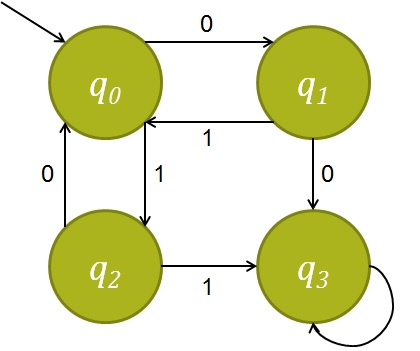
\includegraphics[width=\textwidth,height=0.7\textheight,keepaspectratio]{example}
\end{minipage}}
\begin{minipage}[c][4.5cm]{0.5\textwidth}
 \begin{Verbatim}[fontsize=\tiny]
node top(x : bool; state: int) returns (  );
var
  bias : int;
  guarantee1, guarantee2, guarantee3,
  guarantee4, guarantee5, guarantee_all : bool;
  bias_max : bool;
let
  bias = 0 -> (if x then 1 else -1) + pre(bias);
  bias_max = false ->
	(bias >= 2 or bias <= -2) or pre(bias_max);
  guarantee1 = (state = 0 => (bias = 0));
  guarantee2 = true ->
  	(pre(state = 0) and x) => state = 2;
  guarantee3 = true ->
  	(pre(state = 0) and not x) => state = 1;
  guarantee4 = bias_max => state = 3;
  guarantee5 = state = 0 or state = 1 or state = 2 or 
  		state = 3;
  guarantee_all = guarantee1 and guarantee2 and
  		guarantee3 and guarantee4 and 
  		guarantee5;
  --%PROPERTY guarantee_all;
  --%REALIZABLE x;
tel;
 \end{Verbatim}
\end{minipage}
\caption{Automaton and Requirements for running example}
\vspace{-1em}
\label{fg:example}
\end{figure}

The realizability check on this example succeeds with a k-inductive
proof of length $k = 1$. The two corresponding
$\forall\exists$-formulas ($k=0$ for the base check and $k=1$ for the
inductive check) are valid, and thus \aeval extracts two witnessing
Skolem functions that effectively describe assignments to the local
variables of the specification, as well as to \texttt{state} (see
Appendix~\ref{app:ex} for the particular formulas).

The Skolem functions are used to construct the final implementation
following the outline provided in Template~\ref{alg:synt}. 
The main idea is to redefine each variable in the model
as an array of size equal to $k$ and
to use the $k$-th element of each array as the corresponding output of the call
to $k$-th Skolem function. After this initialization process, we use an infinite
loop to assign new values to the element corresponding to the last Skolem
function, to cover the inductive step of the original proof.

The final code, a snippet of which is presented below, takes 144 lines%
\footnote{Due to the space constraints, full file can be found at \url{http://www.inf.usi.ch/phd/fedyukovich/extended_example.c}}.
Since each Skolem is represented by an $\mathit{ite}$-statement (to be explained in Sect.~\ref{sec:aeval}), each its branch is further encoded into a C-code, for example:

\begin{figure}[h]
\vspace{-2em}
\begin{lstlisting}[language=C]{Name=test2}
if (((x[1] && (-1 == bias[0])) || (!x[1] && (1 == bias[0])))
     && !bias_max[0] 
     && (state[0] != 0 || !x[1]) && (!state[0] != 0 || x[1])) {
  bias_max[1] = 0; bias[1] = 0; state[1] = 0;
}
\end{lstlisting}%
\vspace{-2em}
\end{figure}%


Recall that the user-defined model specifies explicitly two transitions (via \texttt{guarantee2} and \texttt{guarantee3}) only, while the set of implicitly defined transitions (via \texttt{guarantee1} and \texttt{guarantee4}) is incomplete.
For example, the model does not specify an incoming transition to (\texttt{state = 0}).
In contrast, the synthesized implementation turns all implicit transitions into explicit ones which makes them able to execute, and furthermore adds the missing ones (e.g., as in the aforementioned snippet, from \texttt{state = 1} to \texttt{state = 0}).

%%% Local Variables:
%%% mode: latex
%%% TeX-master: "document"
%%% End:

\newcommand{\such}{\,.\,}
\newcommand{\vx}{\vec{x}}
\newcommand{\vy}{\vec{y}}
\newcommand{\Land}{\bigwedge}
\newcommand{\Lor}{\bigvee}
\newcommand{\mbp}{\mathit{MBP}}
\newcommand{\unsat}{\textsc{unsat}}
\newcommand{\sat}{\textsc{sat}}
\newcommand{\valid}{\textsc{valid}\xspace}
\newcommand{\invalid}{\textsc{invalid}\xspace}
\newcommand{\isSat}{\textsc{isSat}\xspace}
\newcommand{\isUnSat}{\textsc{isUNSAT}\xspace}
\newcommand*\rfrac[2]{{}^{#1}\!/_{#2}}
\newcommand{\tuple}[1]{\langle #1 \rangle}       % tuple (in mathmode)

\newcommand{\aevalalgorithm}{%
\begin{algorithm2e}[tb]
\SetAlgoSkip{}
\SetKwFor{While}{forever}{do}{}
%\SetAlgoNoLine
\SetKw{KwContinue}{continue}
\KwIn{$S(\vx), \exists \vy \such T(\vx,\vy)$.}
\KwOut{Return value $\in \{\valid, \invalid\}$ of ${S(\vx)\!\! \implies\!\! \exists \vy \such T(\vx,\vy)}$.}
\KwData{$\textsc{SmtSolver}$, counter $i$, models $\{m_i\}$, MBPs $\{T_{i}(\vx)\}$, conditions $\{\phi_i({\vx,\vy})\}$.}
\BlankLine
$\textsc{SmtAdd}(S(\vx))$; \\
$i \gets 0$; \\
\While{}{
$i$++; \\
%$res \leftarrow \textsc{SmtSolve}()$\label{alg:check_unsat_s}; \\
\lIf(\label{alg:returnUnsat}){$(\isUnSat(\textsc{SmtSolve}()))$}{\Return \valid }
$\textsc{SmtPush}()$; \\
$\textsc{SmtAdd}(T(\vx,\vy))$; \\
%$res \gets \textsc{SmtSolve}()$\label{alg:find_matching_ass};\\
\lIf(\label{alg:returnSat}){$(\isUnSat(\textsc{SmtSolve}()))$}{\Return \invalid }
$m_i \gets \textsc{SmtGetModel}()$\label{alg:model};\\ 
%$E \leftarrow extrapolate(m)$;\\
$(T_{i},\phi_i({\vx,\vy}))\! \gets\! \textsc{GetMBP}(\vy, m_i, T(\vx,\vy)))$\label{alg:proj};\\
$\textsc{SmtPop}()$;\\
$\textsc{SmtAdd}(\neg {T_{i}})$\label{alg:block}; \\
}
%\Return $res$;
\caption{\aeval \Big($S(\vx), \exists \vy \such T(\vx,\vy)$\Big), cf.~\cite{fedyukovich2015automated} }
\label{alg:ae_val}
\end{algorithm2e}
}

\newcommand{\localfactoralg}{%
\begin{algorithm2e}[t!]
\SetAlgoSkip{}
\SetInd{0.4em}{0.4em}
\SetKwFor{ForAll}{forall}{do}{}
\SetKwFor{For}{for}{do}{}
\KwIn{$y_j \in \vy$, local Skolem relation $\phi(\vx,\vy) = \Land_{y_j \in \vy}(\psi_{y_j}(\vx,y_{j},\ldots, y_{n}))$, Skolem functions $y_{j+1} = f_{j+1}(\vx),\ldots, y_{n} = f_{n}(\vx)$.}
\KwData{Factored formula $\pi_{y_j}(\vx,y_{j}) = L_{y_j} \land U_{y_j} \land M_{y_j} \land V_{y_j} \land E_{y_j} \land N_{y_j}$; assuming (for simplicity of presentation) that $M_{y_j} = \varnothing \land  V_{y_j} = \varnothing$.}
\KwOut{Local Skolem function $y_j = f_j(\vx)$.}
\BlankLine
\For{$(i = n; i > j; i++)$}{
  $\psi_{y_j}(\vx,y_{j},\ldots,y_{n}) \gets \textsc{Substitute}(\psi_{y_j}(\vx,y_{j},\ldots,y_{n}) , y_i, f_i(\vx))$\label{alg:loc_subst};\\
}
\BlankLine

$\pi_{y_j}(\vx,y_{j}) \gets \psi_{y_j}(\vx,y_{j},\ldots,y_{n})$\label{alg:elim_compl};\\
\BlankLine

\lIf(){$(E_{y_j} \neq \varnothing)$}{\Return $E_{y_j}$}

$\pi_{y_j}(\vx,y_{j}) \gets \textsc{Merge}(L_{y_j}, \mathit{MAX}, \pi_{y_j}(\vx,y_{j}))$;\\
$\pi_{y_j}(\vx,y_{j}) \gets \textsc{Merge}(U_{y_j} , \mathit{MIN}, \pi_{y_j}(\vx,y_{j}))$;\\
\BlankLine

\lIf(){$(U_{y_j} = \varnothing \land N_{y_j} = \varnothing)$}{\Return $\textsc{Rewrite}(L_{y_j} , \mathit{GT}, \pi_{y_j}(\vx,y_{j}))$}

\lIf(){$(L_{y_j} = \varnothing  \land N_{y_j} = \varnothing)$}{\Return $\textsc{Rewrite}(U_{y_j} , \mathit{LT}, \pi_{y_j}(\vx,y_{j}))$}
\BlankLine

\lIf(){$(N_{y_j} = \varnothing)$}{\Return $\textsc{Rewrite}(L_{y_j} \land U_{y_j} , \mathit{MID}, \pi_{y_j}(\vx,y_{j}))$}

\Return $\textsc{Rewrite}(L_{y_j} \land U_{y_j} \land N_{y_j}, \mathit{FMID}, \pi_{y_j}(\vx,y_{j}))$\label{alg:loc_inst};\\
\caption{$\textsc{ExtractSkolemFunction}(y_j, \phi(\vx,\vy)$)}
\label{alg:loc}
\end{algorithm2e}
}

\section{Witnessing existential quantifiers with \aeval}
\label{sec:aeval}

Quantifier elimination is a decision procedure that turns a quantified formula into an equivalent quantifier-free formula.
In addition, the quantifier elimination algorithms are often able to discover a Skolem function that represents witnesses for the existentially quantified individual variables (e.g.,~\cite{DBLP:conf/cav/BalabanovJ11,DBLP:journals/sttt/KuncakMPS13,KLXJOIA,Chakraborty15}).
%
Various tasks in verification and synthesis~\cite{DBLP:conf/fmcad/CimattiGMT13,DBLP:conf/popl/BeyeneCPR14,DBLP:conf/nfm/GasconT14} rely on efficient techniques to remove existential quantifiers from formulas in first order logic, thus adjusting the task to be decided by an SMT solver.
In particular, \emph{functional synthesis} aims at computing a function that meets a given input/output relation.
A function with an input $x$ and an output $y$, specified by a relation $f(x,y)$, can be constructed as a by-product of deciding validity of the formula $\forall x \exists y \such f(x,y)$.
Due to a well-known \emph{AE-paradigm} (also referred to as \emph{Skolem paradigm}~\cite{DBLP:conf/popl/PnueliR89}),
the formula $\forall x \exists y \such f(x,y)$ is equivalent to the formula $\exists \mathit{sk} \; \forall x \such f(x, \mathit{sk}(x))$, which means existence of a Skolem function $\mathit{sk}$, such that $f(x,\mathit{sk}(x))$ holds for every $x$.
Thus the key feature in modern quantifier elimination approaches is their ability to produce witnessing Skolem function.

In the rest of the section, we briefly describe the prior work on \aeval to be able (in Sect.~\ref{sec:new}) to present the key contributions on delivering Skolem functions appropriate for the program synthesis from proofs of realizability.

\subsection{Model-Based Projection for Linear Rational Arithmetic}
\label{sec:mbp}

Quantifier elimination of a formula $\exists \vy \such T(\vx,\vy)$ is an expensive procedure that typically proceeds by enumerating all models of an extended formula $T(\vx,\vy)$.
However, in some applications, the quantifier-free formula, fully equivalent to $\exists \vy \such T(\vx,\vy)$, is not even needed.
Instead, it is enough to operate by (possibly incomplete) sets of models.
This idea relies on some notion of projection that under-approximates existential quantification.
In this section, we consider a concept of Model-Based Projections (MBP), recently proposed by~\cite{komuravelli2014smt,Dutertre}.

%In the following, we use vector notation to denote sets of variables (and set-theoretic operators of \emph{subset} $\vu \subseteq \vx$, \emph{complement} $\vx_{\vu} = \vx \setminus \vu$, \emph{union} $\vx = \vu \cup \vx_{\vu}$).
\begin{definition}
\label{def:mbp}
An $\mathit{MBP}_{\vy}$ is a function from models of
$T(\vx,\vy)$ to $\vy$-free formulas
iff:
\begin{gather}
\text{if }m\models T(\vx,\vy) \text{ then } m\models \mathit{MBP}_{\vy}(m,T) \label{mbp.cond1}\\
\mathit{MBP}_{\vy}(m,T) \!\implies\! \exists \vy \such T(\vx,\vy) \label{mbp.cond2}
\end{gather}
\end{definition}

There are finitely many MBPs for fixed  $\vy$ and $T$ and different models $m_1,\ldots,m_n$ (for some $n$):
$T_{1}(\vx),  \ldots, T_{n}(\vx)$, such that
$\exists \vy \such T(\vx,\vy) = \Lor_{i=1}^{n} T_{i}(\vx)$. 

A possible way of implementing an MBP-algorithm was proposed in~\cite{komuravelli2014smt}.
It is based on Loos-Weispfenning (LW)  quantifier-elimination method~\cite{loos1993applying} for Linear Rational Arithmetic (LRA).
Consider formula $\exists \vy \such T(\vx,\vy)$, where $T$ is quantifier-free.
In our simplified presentation,
$\vy$ is singleton, $T$ is in Negation Normal Form (that allows the operator $\neg$ to be applied only to variables), and $y$ appears in the literals only of the form ${y=e}$, ${l<y}$ or ${y<u}$, where $l,u,e$ are $y$-free.
LW states that the equation~\eqref{eq:formula_rewrite} holds:

\begin{equation}
  \exists y \such T (\vx) \equiv \Big( \Lor_{(y = e) \in \mathit{lits}(T)}{T[e]} \lor
  	\Lor_{(l < y) \in \mathit{lits} (T)}{T [l + \epsilon]} \lor
	T[-\infty] \Big)\label{eq:formula_rewrite}
\end{equation} 
\smallskip  

In~\eqref{eq:formula_rewrite}, $\mathit{lits}(T)$ denote the set of literals of $T$, $T[\cdot]$ stands for a \emph{virtual substitution} for the literals containing $y$.
In particular, $T[e]$ substitutes exact values of $y$ ($y=e$), $T[l+\epsilon]$ substitutes the intervals ($l < y$) of possible values of $y$, $T[-\infty]$ substitutes the rest of the literals.
Consequently, a function $\mathit{LRAProj_{T}}$ is an implementation of the $\mathit{MBP}$ function for~\eqref{eq:formula_rewrite}:%
%
\begin{equation}
\begin{aligned}
\label{case:proj_define}
&\mathit{LRAProj}_{T}(m) = \left\{
\begin{array}{ll}
T[e], 			& \mbox{if}\ (y=e) \in \mathit{lits}(T) \land 
			m \models (y = e)\\
T[l+ \epsilon],	& \mbox{else if}\ (l < y) \in \mathit{lits}(T) 
			\land m \models (l < y) \land \\
			& \forall (l'\!<\!y)\!\in\!\mathit{lits}(T) \such \!m\!\models\!\big((l'\!<\!y)\!\!\implies\!\!(l'\! \le\! l)\big)\\
T[-\infty], 		& \mbox{otherwise}	
\end{array}
\right.
\end{aligned}
\end{equation}





\subsection{Validity and Skolem extraction}
\label{sim:check}

\aevalalgorithm  

Skolemization (i.e., introducing Skolem functions) is a well-known
technique for removing existential quantifiers in first order formulas.
%More specifically:
%
%\begin{definition}[cf.~\cite{skolem}]
%\label{def:sk_fun}
Given a formula ${ \exists y \such \psi(\vx, y)}$,
a~\emph{Skolem function} for $y$, $\mathit{sk}_{y}(\vx)$ is a function such that
$\exists y \such \psi(\vx,y)\!\iff\!\psi (\vx, \mathit{sk}_{y} (\vx))$.
%\end{definition}
We generalize the definition of a Skolem function for the case of a
vector of existentially quantified variables $\vy$, by relaxing the
relationships between elements of $\vx$ and $\vy$.
Given a formula ${\exists \vy \such \Psi(\vx, \vy)}$, a~\emph{Skolem relation} for $\vy$ is a relation ${\mathit{Sk}_{\vy} (\vx, \vy)}$ such that 1) $\mathit{Sk}_{\vy} (\vx, \vy) \implies \Psi (\vx, \vy)$ and 2) $\exists \vy \such \Psi(\vx, \vy)\!\iff\!\mathit{Sk}_{\vy} (\vx, \vy)$.
  

The algorithm \aeval for deciding validity and Skolem extraction assumes that a formula $\Psi$ can be transformed
into the form ${\exists \vy \such \Psi(\vx, \vy)} \equiv {S(\vx)
  \!\implies\! \exists \vy \such T(\vx,\vy)}$, where $S(\vx)$ has only
existential quantifiers, and $T(\vx, \vy)$ is quantifier-free.
%
\aeval partitions
the formula, and searches for a witnessing local Skolem relation of
each partition.  \aeval iteratively constructs a set of MBPs $\{T_i(\vx)\}$, each of which 
is connected with a so called local Skolem relation $\phi_i(\vx,\vy)$, such that
$\phi_i(\vx,\vy) \!\implies\! (T_{i}(\vx) \!\iff\!
  T(\vx,\vy))$ (i.e., that make the corresponding projections equisatisfiable with $T$).
While the pseudocode of \aeval is shown in Alg.~\ref{alg:ae_val}, we refer the reader to~\cite{fedyukovich2015automated} for
more detail.

%\aeval is shown in Alg.~\ref{alg:ae_val}.  Given formulas
%$S(\vx)$ and ${\exists \vy \such T(\vx, \vy)}$, it
%decides validity of ${S(\vx)\! \implies\! \exists \vy \!\such\!
%  T(\vx, \vy)}$.  \aeval enumerates the
%models of $S \land T$ and blocks them from $S$.
%In each iteration $i$, it first checks whether
%$S$ is non-empty (line~3) and then looks for a model $m_i$ of $S
%\land T$ (line~\ref{alg:model}).  If $m_i$ is found, \aeval
%gets a projection $T_i$ of $T$ based on $m_i$ (line~\ref{alg:proj})
%and blocks all models contained in $T_i$ from $S$
%(line~\ref{alg:block}).  The algorithm iterates until either it
%finds a model of $S$ that can not be extended to a
%model of $T$ (line~\ref{alg:returnSat}), or all models of $S$
%are blocked (line~\ref{alg:returnUnsat}). In the first case, the input
%formula is invalid. In the second case, every model of $S$ has been extended
%to some model of $T$, and the  formula is valid. 

\newcommand{\skolemcases}{%
\begin{equation}
\label{case:skolem}
\mathit{Sk}_{\vy} (\vx, \vy) \equiv
\begin{cases}
  \phi_{1} (\vx, \vy)  & \text{if } T_1 (\vx) \\
    \phi_{2} (\vx, \vy)  & \text{else if } T_2 (\vx)\\
  \cdots &\text{\qquad else }\cdots \\
  \phi_{n} (\vx, \vy) & \text{\qquad\qquad else } T_n (\vx) \\
\end{cases}
\end{equation}
}

A Skolem relation
${\mathit{Sk}_{\vy} (\vx, \vy)}$ by \aeval maps each
model of $S(\vx)$ to a corresponding model of $T(\vx,\vy)$.
Intuitively, $\phi_i$ maps each model of $S \land T_{i}$ to a model of $T$.
Thus, in order to define the  Skolem relation $\mathit{Sk}_{\vy}(\vx, \vy)$ it is enough to 
match each $\phi_i$ against the corresponding $T_{i}$:

\skolemcases


\subsection{Refining Skolem Relations into Skolem Functions}
\label{sec:new}

\localfactoralg


Since \aeval is an extension of the MBP-algorithm mentioned in Sect.~\ref{sec:mbp},
each $\phi_i$ (in~\eqref{case:skolem}) is constructed from the substitutions made in $T$ to produce $T_{i}$.
Furthermore, 
%(is a condition under which $T$ is equisatisfiable with $T_{i}$).
%We assume that each $\phi_i$ is in the Cartesian form, i.e., a conjunction of
%terms, in which each $y_j \in \vy$ appears at most once:
%\begin{equation}
%\label{eq:phi_conj}
%\phi_i(\vx,\vy) = \Land_{y_j \in \vy}(\psi_{y_j}(\vx,y_{j},\ldots,y_{n}))
%\end{equation}
%
%By construction, each local Skolem relation $\phi(\vx,\vy)$ has a form $\Land_{y_j \in \vy}(\psi_{y_j}(\vx,y_{j},\ldots,y_{n}))$.
%Since
each MBP in \aeval is constructed iteratively for each variable $y_j \in \vy$.
Thus, $y_j$ may depend on the variables of $y_{j+1},\ldots, y_{n}$ that are still not eliminated in the current iteration $j$.
%Each $\psi_{y_j}(\vx,y_{j},\ldots,y_{n})$ is the conjunction $\psi_{y_j}(\vx,y_{j},\ldots,y_{n}) = \Land_{i}(cl_i(\vx,y_{j},\ldots,y_{n}))$, where each $cl_i$ is  an (in)equality.

Inequalities in a Skolem relation are the enemies \arie{enemies?!} of program synthesis.
Indeed, the final implementation should contain assignments to each
existentially quantified variable, which are in general difficult to
get. \arie{What is meant by ``difficult''. Difficult computationally,
  difficult for the current algorithm, etc?}
The Skolem relation provided by \aeval should be post-processed to get rid of inequalities.
We formalize this procedure as finding a Skolem function $f_{y_j}(\vx)$ for each $y_j\in \vy$, such that $(y_j = f_{y_j}(\vx)) \!\implies\! \exists y_{j+1},\ldots,y_{n} \such \psi_{y_j}(\vx,y_{j},\ldots,y_{n}) $.
The key idea is presented in Alg.~\ref{alg:loc}.
The algorithm is applied separately for each $y_j \in \vy$, starting from $y_n$ to $y_1$.
For each $y_j$, assume, we already established Skolem functions $f_{j+1}(\vx),\ldots,f_{n}(\vx)$ for variables $y_{j+1},\ldots,y_n$ in the previous runs of the algorithm. 
%
First, the algorithm substitutes each appearance of variables $y_{j+1},\ldots, y_{n}$ in $\psi_{y_j}$ by $f_{n}(\vx),\ldots,f_{j+1}(\vx)$.
%If for some variable there is no Skolem function to substitute, the algorithm halts with nothing (line~\ref{alg:loc_ret_none}).
Second, %the algorithm uses standard LRA-rules to normalize $\pi_{y_j}(\vx,y_{j})$ into the form $\Land_k \big(y_{j} \sim f_k(\vx)\big)$, i.e., conjunction of
%expressions, left-hand-sides of which are reserved for $y_j$ and ${\sim
%\in \{<, \le, =, \ge, >\}}$.
%For this, it uses the method \textsc{Rewrite} (line~\ref{alg:loc_rewrite}) that rewrites each clause using the following rule (where $g,h$ - are functions over $\vx$, $p,q$ - rational numbers, $\mathit{sgn}$ - a function, returning the sign of the rational number):
%
%\begin{equation}
%{\Big( (g(\vx)+ p\!\times\!y_j}) \sim ( {h(\vx) + q\!\times\!y_j})\Big) \!\implies\! \Big(\big(\mathit{sgn}(p-q)\times y_j \big) \sim \big( -\frac{g(\vx)}{|p-q|} + \frac{h(\vx)}{|p-q|} \big)\Big)  \notag
%\end{equation}
%Finally 
the algorithm gets rid of inequalities by transforming them into
equalities, thus producing a Skolem function. \arie{The first part
  (line~2) is clear, the second part is not. Elaborate more which part
  of the algorithm are responsible for which inequality
  elimination. The sets $L$, $U$, $M$, $V$, $E$, $N$, are not
  defined. It is not clear why $M$ and $V$ are present but assumed to
  be empty.}
In the rest of the section, we show several fundamental rules and properties behind this operation.
For simplicity, we omit some straightforward details on dealing with
non-strict inequalities ($y_j \ge l(\vx)$ and $y_j \le u(\vx)$) since
they are similar strict inequalities ($y_j > l(\vx)$ and $y_j < u(\vx)$).

%If there are exist some, $f(\vx)$ defines some interval for the values for $y_j$.
%Method \textsc{SkolemFunction} obtains equalities 
%rewrites each clause using the following rules:

\grigory{the rest can be compressed if needed}.

\begin{lemma}
After all substitutions at line~\ref{alg:elim_compl} of Alg.~\ref{alg:loc}, each $\psi_{y_j}(\vx,y_{j},\ldots,y_{n})$ is a conjunction of the form
$L_{y_j} \land U_{y_j} \land M_{y_j} \land V_{y_j} \land E_{y_j} \land N_{y_j}$ where
%
$L_{y_j} = \Land_{l}(y_j > l(\vx))$, 
$U_{y_j} = \Land_{u}(y_j < u(\vx))$, 
$M_{y_j} = \Land_{l}(y_j \ge l(\vx))$, 
$V_{y_j} = \Land_{u}(y_j \le u(\vx))$, 
$E_{y_j} = \Land_{e}(y_j = e(\vx))$, 
$N_{y_j} = \Land_{n}(y_j \neq n(\vx))$.
%
\end{lemma}
\begin{proof}
Follows directly from~\eqref{case:proj_define}.
\qed
\end{proof}

The procedure to extract a Skolem function out of a Skolem relation proceeds by analyzing terms in $L_{y_j}$, $U_{y_j}$, $M_{y_j}$, $V_{y_j}$,$E_{y_j}$ and $N_{y_j}$.
If there is at least one conjunct $(y_j = e(\vx)) \in E_{y_j}$ then $(y_j = e(\vx))$ itself is a Skolem function.
Otherwise, the algorithm creates it from the following primitives.

\begin{definition}
Let $l(\vx)$ and $u(\vx)$ be two linear terms,
then operators $\mathit{MAX}$, $\mathit{MIN}$, $\mathit{MID}$, $\mathit{LT}$, $\mathit{GT}$ are defined as follows:
\begin{align*}
\mathit{MAX}(l, u) (\vx) &= ite (l (\vx) < u (\vx), u(\vx), l(\vx)) \notag &
\mathit{MIN}(l, u) (\vx) &= ite (l (\vx) < u (\vx), l(\vx), u(\vx)) \notag \\
\mathit{LT} (u) (\vx) &= u (\vx) -1 \notag &
\mathit{GT} (l) (\vx) &= l (\vx) + 1 \notag \\
\mathit{MID}(l, u) (\vx) &= \frac{l(\vx) + u(\vx)}{ 2} \notag 
\end{align*}
\end{definition}

\begin{lemma}
If $L_{y_j}$ consists of $n>1$ conjuncts then it is equivalent to $y_j > \mathit{MAX} (l_1, \mathit{MAX} (l_2,\ldots \mathit{MAX} (l_{n-1}, l_n) )) (\vx)$.
If $U_{y_j}$ consists of $n>1$ conjuncts then it is equivalent to $y_j < \mathit{MIN} (u_1, \mathit{MIN} (u_2,\ldots \mathit{MIN} (u_{n-1}, u_n) ))(\vx)$.
%If  $M_{y_j}$ consists of $n>1$ conjuncts then it is equivalent to $y_j \ge \mathit{MAX} (l_1, \mathit{MAX} (l_2,\ldots \mathit{MAX} (l_{n-1}$, $ l_n) )) (\vx)$.
%If  $V_{y_j}$ consists of $n>1$ conjuncts then it is equivalent to $y_j \le \mathit{MIN} (u_1$, $\mathit{MIN} (u_2,\ldots \mathit{MIN} (u_{n-1}, u_n) )) (\vx)$.
\end{lemma}
Similar for $M_{y_j}$ and for $V_{y_j}$. From this point on, with out
loss of generality, we assume that each $L_{y_j}$, $U_{y_j}$,
$M_{y_j}$, $V_{y_j}$ have at most one conjunct.\arie{Check}

\begin{lemma}
If $L_{y_j}$ consists of 1 conjunct and the rest of $U_{y_j}$, $M_{y_j} $,$V_{y_j}$,$E_{y_j}$ and $N_{y_j}$ are empty then the Skolem can be rewritten into $y_j = \mathit{GT} (l)(\vx)$.
\end{lemma}
Similar for $U_{y_j}$ (Skolem  rewritten into $y_j = \mathit{MID} (u)(\vx)$).

\begin{lemma}
If $L_{y_j}$, $U_{y_j}$  consist of 1 conjunct each, and the rest of $M_{y_j} $,$V_{y_j}$, $E_{y_j}$ and $N_{y_j}$ are empty then the Skolem can be rewritten into $y_j = \mathit{MID} (l, u)(\vx)$. 
\end{lemma}
Similar for $M_{y_j}$ and $V_{y_j}$, and for combinations with $L_{y_j}$ and $U_{y_j}$.


\begin{lemma}
  \arie{It is not clear where $h$ comes from}
If $L_{y_j}$, $U_{y_j}$ and $N_{y_j}$ consist of 1 conjunct each and the rest of $M_{y_j} $,$V_{y_j}$,$E_{y_j}$ and $N_{y_j}$ are empty then the Skolem can be rewritten into $y_j = \mathit{FMID} (l, u, h)(\vx)$, where%
\begin{align}
\mathit{FMID}(l, u, h) (\vx) = ite (&\mathit{MID}(l, u) (\vx) = h(\vx),  \notag \\
                          &\mathit{MID}(l, \mathit{MID}(l, u)) (\vx), \notag \\
                          &\mathit{MID}(l, u) (\vx)) \notag 
\end{align}
\end{lemma}
Similar for $M_{y_j}$ and $V_{y_j}$. 
For bigger number of conjuncts of $N_{y_j}$, the Skolem gets rewritten
in a similar way cascadically\arie{Not a word}.


\begin{lemma}
If $L_{y_j}$, $N_{y_j}$  consist of 1 conjunct each, and the rest of $M_{y_j} $,$V_{y_j}$, $E_{y_j}$ and $U_{y_j}$ are empty then the Skolem can be rewritten into $y_j = \mathit{FMID} (l, GT(l))(\vx)$. 
\end{lemma}
Similar for $M_{y_j}$.


\begin{lemma}
If $U_{y_j}$, $N_{y_j}$  consist of 1 conjunct each, and the rest of $M_{y_j} $,$V_{y_j}$, $E_{y_j}$ and $L_{y_j}$ are empty then the Skolem can be rewritten into $y_j = \mathit{FMID} (LT(u), u)(\vx)$. 
\end{lemma}
Similar for $V_{y_j}$.


\begin{theorem}[Soundness]
Iterative application of Alg.~\ref{alg:loc} to all variables $y_n,\ldots,y_1$ returns a local Skolem function to be used in~\eqref{case:skolem}.
\end{theorem}
\begin{proof}
Follows from the case analysis that applies the lemmas above.
\qed
\end{proof}

%%% Local Variables:
%%% mode: latex
%%% TeX-master: "document"
%%% End:

\section{Case Studies}

\subsection{A simple controller example}

In this section, we provide an illustrative example of how the synthesis
algorithm creates a simple implementation from specifications describing the
constraints that a controller must meet. The specification is written in the
Lustre language, and can be seen in Figure~\ref{fig:example}. The controller
is used to maintain an appropriate level of \textit{speed} at each next step of
its execution, using two auxillary signals, called \textit{plus} and
\textit{minus} to help determine future decisions on acceleration or deceleration. There is
only one input to this example, called \textit{diff}, and is used to compute
the amount by which the \textit{speed} value changes with each new state.

The specification is composed of an auxillary node called Sofar, that is a
custom operation on a boolean variable to capture whether it has been
historically true up to and including the current step. The rest of the nodes
defined essentially cover the assumptions and the guarantees that the contract
contains. The node \textit{Environment} is used to describe restrictions on the
input variable \textit{diff}, while the system's correct response is captured by the
node \textit{Property}. The \textit{top} node of the specification is used as
the main block of this program, and combines the two constraints to effectively
define the structure of the final property that the system should be respecting
at all states during its execution.

\andreas{add discription of Controller node. Add text for synthesis case}

 \begin{figure}[H]
 \begin{lstlisting}[basicstyle=\ttfamily\footnotesize]
--
-- Source Bertrand Jeannet, NBAC tutorial
--

node Sofar( X : bool ) returns ( Sofar : bool );
let
    Sofar = X -> X and pre Sofar;
tel

node Environment(diff: int; plus,minus: bool) returns (ok: bool);
let
  ok = (-4 <= diff and diff <= 4) and 
     (if (true -> pre plus) then diff >= 1 else true) and
     (if (false -> pre minus) then diff <= -1 else true);
tel

node Controller(diff: int) returns (speed: int; plus,minus: bool);
let
  speed = 0 -> pre(speed)+diff;
  plus = speed <= 9;
  minus = speed >= 11;
tel

node Property(speed: int) returns (ok: bool);
var cpt: int;
    acceptable: bool;
let
  acceptable = 8 <= speed and speed <= 12;
  cpt = 0 -> if acceptable then 0 else pre(cpt)+1;
  ok = true -> (pre cpt<=7);
tel

--@ ensures OK;
node top(diff:int) returns (OK: bool);
var speed: int; 
    plus,minus,realistic: bool;
let
  (speed,plus,minus) = Controller(diff);
  realistic =  Environment(diff,plus,minus);

  OK = Sofar( realistic and 0 <= speed and speed < 16 ) => Property(speed);
  --%PROPERTY OK;
  --%MAIN;
tel 
\end{lstlisting}
 \caption{Specification for a Controller in Lustre}
 \label{fig:example}
 \end{figure}
 

\label{sec:cstudies}


\section{Related Work}

Research in the field of program synthesis attributes its origins in the 1970s,
when Zohar Manna and Richard Waldinger first introduced a synthesis procedure
using theorem proving.~\cite{manna1971toward}. Almost two decades later, Amir
Pnueli and Roni Rosner were the first to propose a way to synthesize
implementations for temporal specifications~\cite{DBLP:conf/popl/PnueliR89}. This work also
involved the first formal definition of a reactive system's realizability (or implementability) and
introduces a \emph{Skolem paradigm} on which we heavily rely in this work.
%i.e., the formula $\forall x \exists y \such f(x,y)$ is equivalent to the formula $\exists \mathit{sk} \; \forall x \such f(x, \mathit{sk}(x))$, which means existence of a Skolem function $\mathit{sk}$, such that $f(x,\mathit{sk}(x))$ holds for every $x$.


Since then, a vast variety of techniques have been developed. Efficient
algorithms were proposed for subsets of propositional LTL
\cite{Klein10,tomita2016safraless,ehlers2010symbolic,cheng2016structural} simple
LTL formulas \cite{Bohy12,hagihara2016simple,Tini03}, as well as other temporal
logics \cite{benevs2012factorization,monmege2016real,Hamza10}, such as SIS \cite{Aziz95}.
Component-based approaches have also been explored in~\cite{Chatterjee07,dammyou}.

Sumit Gulwani in 2010 published a survey on which he discribed the
potential future directions of program synthesis research~\cite{gulwani2010dimensions}.
The approaches that have been proposed are many, and differ on many aspects,
either in terms of the specifications that are being exercised, or the reasoning
behind the synthesis algorithm itself. Template-based
synthesis~\cite{srivastava2013template} is focused on the exploration of
programs that satisfy a specification that is refined after each
iteration, following the basic principles of deductive synthesis. Inductive
synthesis is an active area of research where the main goal
is the generation of an inductive invariant that can be used to describe the
space of programs that are guaranteed to satisfy the given
specification~\cite{flener2001inductive}.
This idea is mainly supported by the use of SMT solvers to guide the invariant
refinement through traces that violate the requirements, known as
counterexamples. Recently published work on extending SMT solvers with
counterexample-guided synthesis shows that they can eventually be
used as an alternative to solving the problem under certain domains of
arithmetic~\cite{reynoldscounterexample}. Reactive synthesis has also
been explored in the context involving propositional formulas for safety
specifications~\cite{bloem2016satisfiability}. Finally, functional synthesis is
used in applications where only a partial implementation exists, and the user needs an automated way to complete the missing parts of the program~\cite{kneuss2013integrating}.

A rather important contribution in the area is the recently published work by
Leonid Ryzhyk and Adam Walker~\cite{ryzhykdeveloping}, where they share their
experience in developing and using a reactive synthesis tool for controllers in
an industrial environment. While the authors emphasize that the research on
program synthesis is still at a very early stage for the technique to be
essential to industrial applications, they note its potential advantages in terms
of improving the overall development cycle of software.

To the best of our knowledge our work is the first complete attempt on providing
a synthesis algorithm for an assume-guarantee framework, using infinite theories.
We take advantage of a sophisticated solver that is able to reason about the
validity of the intermediate formulas that construct a k-inductive proof, as
well as provide witnesses for these formulas through the use of Skolem
functions. The ability to express contracts that support ideas from many
categories of specifications, such as template-based and temporal properties,
increases the potential applicability of this work to multiple subareas on
synthesis research.
\label{sec:related}

%%% Local Variables:
%%% mode: latex
%%% TeX-master: "document"
%%% End:

\section{Future Work}

While our current approach to program synthesis has been shown to be effective
in the contracts that we have exercised, there are yet a lot of interesting ways
to extend and optimize the underlying algorithm, to yield better results in the
future. An important extension is that of supporting additional theories such as
integers, which is currently not supported by AE-VAL's model based projection
technique. To combat the lack of soundness on unrealizable results, and thus
missing potential synthesized implementations, we will be developing a new
algorithm that is mainly based on the idea of generating inductive invariants,
much like the way that is presented in Property Directed Reachability
algorithms. Finally, another potential optimization that could effectively
reduce the algorithm's complexity is the further simplification of the
transition relation that we are currently using, by reducing its complicated
form through the mapping of common subexpressions on different conditional
branches. This will also have a direct impact on the skolem relations retrieved
by AE-VAL, reducing their individual size and improving, thus, the final
implementation in terms of readability as well as its usability as an
intermediate representation to the preferred target language.


\label{sec:futurework}



\section*{Acknowledgments}
This work was funded by DARPA and AFRL under contract 4504789784 (Secure Mathematically-Assured Composition of Control Models), and by NASA under contract NNA13AA21C (Compositional Verification of Flight Critical Systems), and by NSF under grant CNS-1035715 (Assuring the safety, security, and reliability of medical device cyber physical systems).
\bibliography{document}
\bibliographystyle{splncs03}

\end{document}
